
    \subsubsection{Quản lý hoạt động công tác xã hội}

    Module Công tác Xã hội cung cấp các chức năng quản lý toàn diện hoạt động CTXH của sinh viên, bao gồm 6 chức năng chính:

    \begin{enumerate}
        \item \textbf{Quản lý danh mục:} Tạo, cập nhật và phân loại các danh mục hoạt động CTXH.
        \item \textbf{Quản lý hoạt động:} Tạo, chỉnh sửa thông tin hoạt động CTXH (tên, thời gian, địa điểm, số ngày CTXH).
        \item \textbf{Quản lý người tham gia:} Thêm sinh viên (thủ công/Excel), chấm điểm ngày CTXH (thủ công/Excel), xuất danh sách.
        \item \textbf{Cấu hình giới hạn:} Thiết lập số ngày CTXH tối đa theo tổ chức, tự động áp dụng cho tổ chức con.
        \item \textbf{Nhập dữ liệu từ hệ thống cũ:} Nhập số ngày CTXH từ hệ thống cũ bằng file Excel.
        \item \textbf{Xem báo cáo cá nhân:} Sinh viên xem tổng số ngày đã tích lũy, trạng thái đạt/chưa đạt yêu cầu 15 ngày.
    \end{enumerate}

    Trong đó, 3 chức năng đầu (Quản lý danh mục, hoạt động, người tham gia) có use case diagram chi tiết riêng do độ phức tạp cao. 3 chức năng còn lại (Cấu hình giới hạn, Nhập dữ liệu cũ, Xem báo cáo cá nhân) được thể hiện trong diagram tổng quát và chỉ mô tả bằng bảng specification do tính đơn giản.

    % Diagram tổng quát Module CTXH
    \begin{figure}[H]
        \centering
        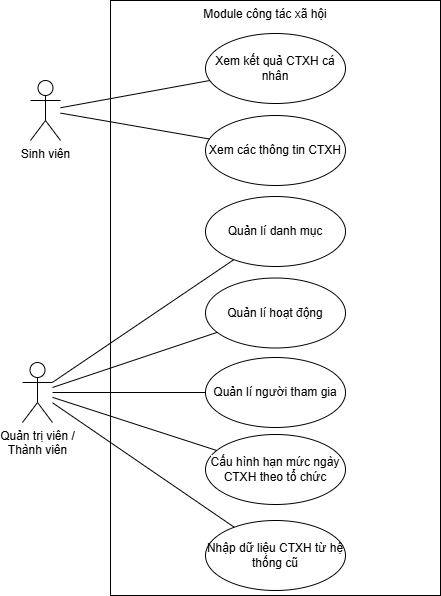
\includegraphics[width=0.6\linewidth]{Images/use-case-diagram/UC07_tong_quat.png}
        \vspace{0.3em}
        \captionsetup{skip=8pt} % tăng khoảng cách ảnh–caption
        \caption{UC07 - Quản lý hoạt động Công tác Xã hội (bao gồm UC7.4 - Cấu hình giới hạn, UC7.5 - Xem báo cáo cá nhân, UC7.6 - Nhập dữ liệu hệ thống cũ)}
        \label{fig:uc07-tong-quat}
    \end{figure}

    % UC7.1 - Quản lý danh mục
    \newpage
    \begin{figure}[H]
        \centering
        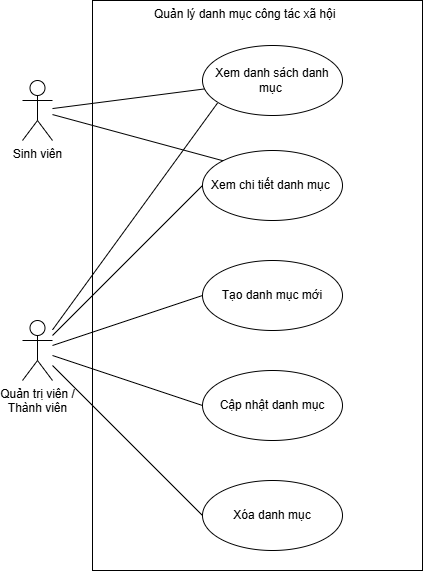
\includegraphics[width=0.6\linewidth]{Images/use-case-diagram/UC07_03_danh_muc.png}
        \vspace{0.3em}
        \captionsetup{skip=8pt} % tăng khoảng cách ảnh–caption
        \caption{UC7.1 - Quản lý danh mục công tác xã hội}
        \label{fig:uc07-01}
    \end{figure}

    \newpage
    \begin{table}[H]
    \renewcommand{\arraystretch}{1.3}
    \begin{tabular}{|m{0.25\textwidth}|m{0.75\textwidth}|}
    \hline
    \textbf{Use Case Name} 
    & \textbf{UC7.1. Quản lý danh mục công tác xã hội} \\ \hline

\textbf{Actors} 
& Quản trị viên, Người dùng \\ \hline

\textbf{Description}
    & Use case này cho phép Quản trị viên/Người dùng quản lý danh mục CTXH để phân loại các hoạt động công tác xã hội. Bao gồm:
    \begin{itemize}
        \item Tạo danh mục mới
        \item Xem danh sách danh mục
        \item Xem chi tiết danh mục và danh sách hoạt động thuộc danh mục
        \item Cập nhật thông tin danh mục
        \item Xóa danh mục
    \end{itemize}
    \\ \hline

    \textbf{Trigger} 
    & Quản trị viên/Người dùng muốn tạo, xem, chỉnh sửa hoặc xóa danh mục để phân loại hoạt động CTXH.
    \\ \hline

    \textbf{Pre-Conditions} 
    & \begin{itemize}
        \item Người dùng đã đăng nhập vào hệ thống
        \item Có các quyền xem và quản lí danh mục công tác xã hội
    \end{itemize}
    \\ \hline

    \textbf{Post-Conditions} 
    & \begin{itemize}
        \item Danh mục được tạo mới, cập nhật hoặc xóa (mềm) trong database
        \item Có thể xem danh sách hoạt động thuộc danh mục
    \end{itemize}
    \\ \hline

    \textbf{Normal Flow} 
    & \textbf{Tạo danh mục mới:}
    \begin{enumerate}
        \item Người dùng click "Tạo danh mục mới", nhập tên và mô tả
        \item Hệ thống validate tên không trống, chưa tồn tại
        \item Tạo danh mục và hiển thị thông báo thành công
    \end{enumerate}

    \textbf{Xem chi tiết:}
    \begin{enumerate}
        \item Người dùng click vào danh mục
        \item Hệ thống hiển thị thông tin danh mục và danh sách hoạt động
    \end{enumerate}

    \textbf{Cập nhật:}
    \begin{enumerate}
        \item Người dùng click "Sửa", chỉnh sửa thông tin
        \item Hệ thống validate và cập nhật danh mục
    \end{enumerate}

    \textbf{Xóa:}
    \begin{enumerate}
        \item Người dùng click "Xóa"
        \item Hệ thống kiểm tra: Nếu có hoạt động thì không cho xóa
        \item Nếu không có hoạt động: Hiển thị xác nhận và xóa mềm
    \end{enumerate}
    \\ \hline
    \end{tabular}
    \end{table}

    \newpage
    \begin{table}[H]
    \renewcommand{\arraystretch}{1.3}
    \begin{tabular}{|m{0.25\textwidth}|m{0.75\textwidth}|}
    \hline
    \textbf{Alternative Flow} 
    & \textbf{Tạo mới:}
    \begin{itemize}
        \item \textbf{4a.} Tên trống: Hiển thị "Tên danh mục không được để trống", quay lại bước 3
        \item \textbf{4b.} Tên đã tồn tại: Hiển thị "Danh mục đã tồn tại", quay lại bước 3
    \end{itemize}

    \textbf{Xem chi tiết:}
    \begin{itemize}
        \item \textbf{2a.} Danh mục không có hoạt động nào: Hiển thị "Chưa có hoạt động nào trong danh mục này"
    \end{itemize}

    \textbf{Cập nhật:}
    \begin{itemize}
        \item \textbf{2a.} Danh mục không tồn tại: Hiển thị lỗi không tìm thấy, quay về danh sách
        \item \textbf{5a.} Tên mới đã tồn tại: Hiển thị "Danh mục đã tồn tại", quay lại bước 3
    \end{itemize}

    \textbf{Xóa:}
    \begin{itemize}
        \item \textbf{2a.} Danh mục có hoạt động: 
        \begin{itemize}
            \item Hiển thị lỗi "Không thể xóa danh mục đã có hoạt động. Vui lòng xóa tất cả hoạt động trước."
            \item Không cho phép xóa
        \end{itemize}
        \item \textbf{4a.} Người dùng click "Hủy": Đóng hộp thoại, không xóa
        \item \textbf{5a.} Không có quyền delete: Hiển thị "Bạn không có quyền xóa danh mục"
    \end{itemize}
    \\ \hline

    \textbf{Exception} 
    & \begin{itemize}
        \item Lỗi database: Hiển thị "Không thể lưu danh mục, vui lòng thử lại"
        \item Mất kết nối: Hiển thị "Lỗi kết nối, vui lòng thử lại sau"
    \end{itemize}
    \\ \hline
    \end{tabular}
    \caption{Bảng mô tả Use Case UC7.1 - Quản lý danh mục công tác xã hội}
    \end{table}

    % ========================================
    % UC7.2 - Quản lý người tham gia
    \newpage
    \begin{figure}[H]
        \centering
        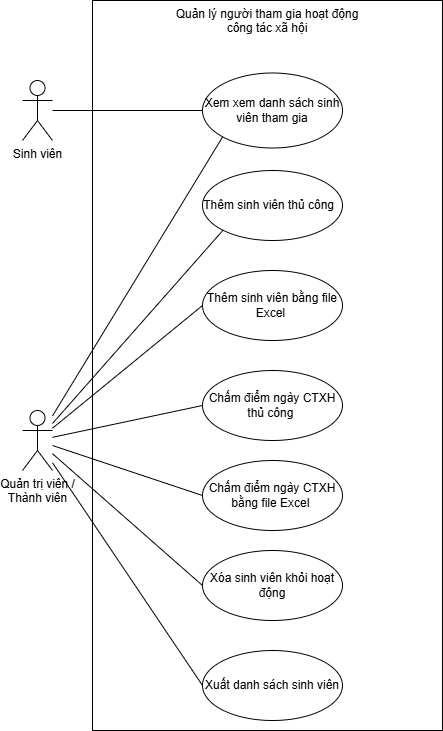
\includegraphics[width=0.8\linewidth]{Images/use-case-diagram/UC07_02_nguoi_tham_gia.png}
        \vspace{0.3em}
        \captionsetup{skip=8pt} % tăng khoảng cách ảnh–caption
        \caption{UC7.2 - Quản lý người tham gia hoạt động}
        \label{fig:uc07-02}
    \end{figure}

    \newpage
    \begin{table}[H]
    \renewcommand{\arraystretch}{1.3}
    \begin{tabular}{|m{0.25\textwidth}|m{0.75\textwidth}|}
    \hline
    \textbf{Use Case Name} 
    & \textbf{UC7.2. Quản lý người tham gia hoạt động} \\ \hline

\textbf{Actors} 
& Quản trị viên, Người dùng \\ \hline

\textbf{Description} 
    & Use case này cho phép quản lý danh sách sinh viên tham gia hoạt động CTXH, bao gồm:
    \begin{itemize}
        \item Xem danh sách sinh viên
        \item Thêm sinh viên thủ công (nhập mã số)
        \item Thêm sinh viên bằng file Excel
        \item Chấm điểm CTXH thủ công
        \item Chấm điểm bằng file Excel
        \item Xóa sinh viên khỏi hoạt động
        \item Xuất danh sách sinh viên
    \end{itemize}
    \\ \hline

    \textbf{Trigger} 
    & Quản trị viên/Người dùng muốn thêm sinh viên vào hoạt động hoặc chấm điểm sau khi hoạt động kết thúc.
    \\ \hline

    \textbf{Pre-Conditions} 
    & \begin{itemize}
        \item Người dùng đã đăng nhập
        \item Có quyền quản lý người tham gia hoạt động công tác xã hội
        \item Hoạt động tồn tại với trạng thái "Đang hoạt động'
    \end{itemize}
    \\ \hline

    \textbf{Post-Conditions} 
    & \begin{itemize}
        \item Bản ghi tham gia hoạt động được tạo hoặc cập nhật trong hệ thống
        \item Số ngày CTXH được cộng vào tổng số ngày CTXH của sinh viên
        \item Sinh viên thấy kết quả trong báo cáo cá nhân
    \end{itemize}
    \\ \hline

    \textbf{Normal Flow} 
    & \textbf{Thêm sinh viên thủ công:}
    \begin{enumerate}
        \item Người dùng nhập mã số sinh viên
        \item Hệ thống validate: sinh viên tồn tại, chưa tham gia
        \item Tạo bản ghi tham gia với trạng thái "Đã đăng ký"
    \end{enumerate}

    \textbf{Chấm điểm thủ công:}
    \begin{enumerate}
        \item Người dùng nhập số ngày (bội 0.5)
        \item Hệ thống validate: số ngày hợp lệ, không vượt giới hạn
        \item Cập nhật số ngày và cộng vào tổng CTXH của sinh viên
    \end{enumerate}

    \textbf{Chấm điểm Excel:}
    \begin{enumerate}
        \item Người dùng tải mẫu và tải lên file Excel
        \item Hệ thống parse file (chunk 500 rows), validate từng row
        \item Hiển thị preview: hợp lệ/lỗi
        \item Cập nhật hàng loạt sau khi xác nhận
    \end{enumerate}
    \\ \hline
    \end{tabular}
    \end{table}

    \newpage
    \begin{table}[H]
    \renewcommand{\arraystretch}{1.3}
    \begin{tabular}{|m{0.25\textwidth}|m{0.75\textwidth}|}
    \hline
    \textbf{Alternative Flow} 
    & \textbf{Thêm sinh viên:}
    \begin{itemize}
        \item \textbf{5a.} Không tìm thấy sinh viên: Hiển thị "Không tìm thấy sinh viên", quay lại bước 4
        \item \textbf{5b.} Sinh viên đã tham gia: Hiển thị "Sinh viên đã tham gia", quay lại bước 4
    \end{itemize}

    \textbf{Chấm điểm thủ công:}
    \begin{itemize}
        \item \textbf{4a.} Số ngày không hợp lệ: Hiển thị lỗi cụ thể, quay lại bước 3
        \item \textbf{4b.} Số ngày vượt giới hạn: Hiển thị "Vượt quá số ngày tối đa của hoạt động", quay lại bước 3
    \end{itemize}

    \textbf{Chấm điểm Excel:}
    \begin{itemize}
        \item \textbf{4a.} File sai định dạng: Hiển thị "Vui lòng sử dụng file .xlsx", quay lại bước 3
        \item \textbf{5a.} Có row lỗi: Đánh dấu lỗi trong preview, chỉ update row hợp lệ
    \end{itemize}
    \\ \hline

    \textbf{Exception} 
    & \begin{itemize}
        \item Hoạt động không ở trạng thái đang hoạt động: "Chỉ thêm sinh viên vào hoạt động đang hoạt động"
        \item File Excel > 10MB: "File quá lớn, tối đa 10MB"
        \item Lỗi database batch update: Rollback transaction, hiển thị lỗi
    \end{itemize}
    \\ \hline
    \end{tabular}
    \caption{Bảng mô tả Use Case UC7.2 - Quản lý người tham gia hoạt động}
    \end{table}

    % ========================================
    % UC7.3 - Quản lý hoạt động
    \newpage
    \begin{figure}[H]
        \centering
        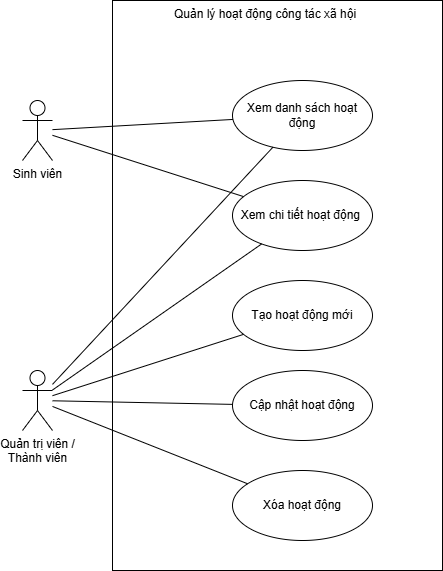
\includegraphics[width=0.7\linewidth]{Images/use-case-diagram/UC07_03_hoat_dong.png}
        \vspace{0.3em}
        \captionsetup{skip=8pt} % tăng khoảng cách ảnh–caption
        \caption{UC7.3 - Quản lý hoạt động công tác xã hội}
        \label{fig:uc07-03}
    \end{figure}

    \newpage
    \begin{table}[H]
    \renewcommand{\arraystretch}{1.3}
    \begin{tabular}{|m{0.25\textwidth}|m{0.75\textwidth}|}
    \hline
    \textbf{Use Case Name} 
    & \textbf{UC7.3. Quản lý hoạt động công tác xã hội} \\ \hline

\textbf{Actors} 
& Quản trị viên, Người dùng \\ \hline

\textbf{Description} 
    & Use case này cho phép quản lý hoạt động CTXH trong hệ thống:
    \begin{itemize}
        \item Tạo hoạt động mới (Nháp/Đang hoạt động)
        \item Xem danh sách hoạt động
        \item Cập nhật thông tin hoạt động
        \item Xóa hoạt động
    \end{itemize}
    \\ \hline

    \textbf{Trigger} 
    & Quản trị viên/Người dùng muốn tạo hoạt động CTXH mới hoặc chỉnh sửa hoạt động hiện có.
    \\ \hline

    \textbf{Pre-Conditions} 
    & \begin{itemize}
        \item Người dùng đã đăng nhập
        \item Có quyền tạo mới hoặc cập nhật hoạt động công tác xã hội
        \item Có ít nhất 1 danh mục trong hệ thống
    \end{itemize}
    \\ \hline

    \textbf{Post-Conditions} 
    & \begin{itemize}
        \item Hoạt động được tạo mới hoặc cập nhật
        \item Trạng thái: Nháp hoặc Đang hoạt động tùy theo cấu hình
        \item Hoạt động hiển thị trong danh sách
    \end{itemize}
    \\ \hline

    \textbf{Normal Flow} 
    & \textbf{Tạo hoạt động mới:}
    \begin{enumerate}
        \item Người dùng nhập thông tin: tên, danh mục, địa điểm, thời gian, số ngày, trạng thái
        \item Hệ thống validate: tên không trống, ngày kết thúc sau ngày bắt đầu, số ngày là bội 0.5
        \item Kiểm tra cấu hình giới hạn: nếu vượt thì cảnh báo nhưng vẫn cho tạo
        \item Lưu hoạt động vào cơ sở dữ liệu
    \end{enumerate}

    \textbf{Cập nhật:}
    \begin{enumerate}
        \item Người dùng chỉnh sửa thông tin hoạt động
        \item Hệ thống validate (tương tự tạo mới) và cập nhật
    \end{enumerate}
    \\ \hline

    \textbf{Alternative Flow} 
    & \textbf{Tạo mới:}
    \begin{itemize}
        \item \textbf{4a.} Tên trống: Hiển thị "Tên không được để trống", quay lại bước 3
        \item \textbf{4b.} Tên trùng: Hiển thị "Hoạt động đã tồn tại trong danh mục", quay lại bước 3
        \item \textbf{4c.} Không có quyền tổ chức: Hiển thị "Không có quyền", quay lại bước 3
        \item \textbf{4d.} Thời gian không hợp lệ: Hiển thị lỗi, quay lại bước 3
        \item \textbf{4e.} Số ngày không hợp lệ: "Số ngày phải là bội của 0.5", quay lại bước 3
        \item \textbf{4f.} Trạng thái đang hoạt động nhưng thiếu thông tin: "Cần đầy đủ địa điểm, thời gian, số ngày", quay lại bước 3
    \end{itemize}

    \textbf{Cập nhật:}
    \begin{itemize}
        \item \textbf{2a.} Hoạt động không tồn tại: Hiển thị lỗi không tìm thấy, quay về danh sách
        \item \textbf{5a.} Validate lỗi: Tương tự tạo mới
    \end{itemize}
    \\ \hline

    \textbf{Exception} 
    & \begin{itemize}
        \item Danh mục không tồn tại: Hiển thị lỗi không tìm thấy danh mục
        \item Lỗi database: Hiển thị "Không thể lưu hoạt động, vui lòng thử lại"
    \end{itemize}
    \\ \hline
    \end{tabular}
    \caption{Bảng mô tả Use Case UC7.3 - Quản lý hoạt động công tác xã hội}
    \end{table}

    % ========================================
    % UC7.4 - Quản lý hạn mức ngày CTXH theo chức
    \newpage
    \begin{table}[H]
    \renewcommand{\arraystretch}{1.3}
    \begin{tabular}{|m{0.25\textwidth}|m{0.75\textwidth}|}
    \hline
    \textbf{Use Case Name} 
    & \textbf{UC7.4. Quản lý hạn mức ngày CTXH theo chức} \\ \hline

\textbf{Actors} 
& Quản trị viên \\ \hline

\textbf{Description}
    & Quản trị viên thiết lập số ngày CTXH tối đa được phép cho từng tổ chức. Cấu hình tự động áp dụng cho tất cả tổ chức con chưa có cấu hình hoặc đang hoạt động.
    \\ \hline

    \textbf{Trigger} 
    & Quản trị viên muốn giới hạn số ngày một hoạt động có thể cấp cho sinh viên theo từng tổ chức.
    \\ \hline

    \textbf{Pre-Conditions} 
    & \begin{itemize}
        \item Người dùng đã đăng nhập
        \item Có quyền cấu hình giới hạn số ngày CTXH
        \item Tổ chức tồn tại trong hệ thống
    \end{itemize}
    \\ \hline

    \textbf{Post-Conditions} 
    & \begin{itemize}
        \item Cấu hình giới hạn được tạo với thông tin tổ chức, số ngày tối đa và trạng thái
        \item Tổ chức con tự động được cập nhật cấu hình
    \end{itemize}
    \\ \hline

    \textbf{Normal Flow} 
    & 
    \begin{enumerate}
        \item Người dùng truy cập "Cấu hình giới hạn", click "Tạo cấu hình"
        \item Chọn tổ chức, nhập số ngày tối đa, chọn trạng thái
        \item Hệ thống validate: số ngày > 0, tổ chức tồn tại
        \item Tạo cấu hình cho tổ chức cha
        \item Tự động áp dụng cho tổ chức con (cấp 1, 2): tạo mới hoặc cập nhật nếu đang hoạt động
        \item Hiển thị "Đã tạo cấu hình và áp dụng cho X tổ chức con"
    \end{enumerate}
    \\ \hline

    \textbf{Alternative Flow} 
    & \begin{itemize}
        \item \textbf{7a.} Số ngày $\leq$ 0: Hiển thị "Số ngày phải > 0", quay lại bước 5
        \item \textbf{7b.} Tổ chức đã có cấu hình đang hoạt động: Hiển thị "Tổ chức đã có cấu hình"
    \end{itemize}
    \\ \hline

    \textbf{Exception} 
    & \begin{itemize}
        \item Tổ chức không tồn tại: Hiển thị lỗi không tìm thấy tổ chức
    \end{itemize}
    \\ \hline
    \end{tabular}
    \caption{Bảng mô tả Use Case UC7.4 - Quản lý hạn mức ngày CTXH theo chức}
    \end{table}

    % ========================================
    % UC7.5 - Xem báo cáo ngày CTXH cá nhân
    \newpage
    \begin{table}[H]
    \renewcommand{\arraystretch}{1.3}
    \begin{tabular}{|m{0.25\textwidth}|m{0.75\textwidth}|}
    \hline
    \textbf{Use Case Name} 
    & \textbf{UC7.5. Xem báo cáo ngày công tác xã hội cá nhân} \\ \hline

\textbf{Actors} 
& Sinh viên \\ \hline

\textbf{Description}
    & Sinh viên xem báo cáo CTXH cá nhân bao gồm tổng số ngày đã tích lũy, trạng thái đạt/chưa đạt, và danh sách chi tiết các hoạt động đã tham gia. Hệ thống tính từ cả ngày mới (hệ thống hiện tại) và ngày cũ (nhập từ hệ thống cũ).
    \\ \hline

    \textbf{Trigger} 
    & Sinh viên muốn kiểm tra tiến độ CTXH, xem đã đạt 15 ngày chưa.
    \\ \hline

    \textbf{Pre-Conditions} 
    & \begin{itemize}
        \item Người dùng đã đăng nhập
        \item Tài khoản sinh viên có mã số sinh viên trong hệ thống
    \end{itemize}
    \\ \hline

    \textbf{Post-Conditions} 
    & Báo cáo CTXH cá nhân hiển thị đầy đủ thông tin
    \\ \hline

    \textbf{Normal Flow} 
    & 
    \begin{enumerate}
        \item Sinh viên click "Báo cáo CTXH của tôi"
        \item Hệ thống lấy mã số, truy vấn: số ngày mới + số ngày cũ, danh sách hoạt động đã tham gia
        \item Tính tổng số ngày, kiểm tra đạt yêu cầu (>= 15 ngày)
        \item Hiển thị báo cáo: thông tin, tổng ngày, trạng thái đạt/chưa đạt, danh sách hoạt động
    \end{enumerate}
    \\ \hline

    \textbf{Alternative Flow} 
    & \begin{itemize}
        \item \textbf{2a.} Sinh viên chưa tham gia hoạt động nào:
        \begin{itemize}
            \item Hiển thị "Bạn chưa tham gia hoạt động CTXH nào"
            \item Hiển thị button "Xem danh sách hoạt động"
        \end{itemize}
        \item \textbf{5a.} Tổng ngày $\geq$ 15:
        \begin{itemize}
            \item Hiển thị badge "Da hoan thanh CTXH"
        \end{itemize}
    \end{itemize}
    \\ \hline

    \textbf{Exception} 
    & Không tìm thấy thông tin sinh viên: Hiển thị lỗi tài khoản không hợp lệ
    \\ \hline
    \end{tabular}
    \caption{Bảng mô tả Use Case UC7.5 - Xem báo cáo ngày công tác xã hội cá nhân}
    \end{table}

    % ========================================
    % UC7.6 - Nhập dữ liệu từ hệ thống cũ
    \newpage
    \begin{table}[H]
    \renewcommand{\arraystretch}{1.3}
    \begin{tabular}{|m{0.25\textwidth}|m{0.75\textwidth}|}
    \hline
    \textbf{Use Case Name} 
    & \textbf{UC7.6. Nhập dữ liệu ngày CTXH từ hệ thống cũ} \\ \hline

\textbf{Actors} 
& Quản trị viên \\ \hline

\textbf{Description}
    & Quản trị viên tải lên file Excel chứa mã số sinh viên và số ngày CTXH từ hệ thống cũ. Hệ thống phân tích, kiểm tra và cập nhật số ngày CTXH từ hệ thống cũ vào hồ sơ sinh viên. Sử dụng khi chuyển đổi dữ liệu từ hệ thống cũ sang hệ thống mới.
    \\ \hline

    \textbf{Trigger} 
    & Quản trị viên muốn nhập dữ liệu CTXH từ hệ thống cũ khi lần đầu triển khai.
    \\ \hline

    \textbf{Pre-Conditions} 
    & \begin{itemize}
        \item Người dùng đã đăng nhập
        \item Có quyền nhập dữ liệu từ hệ thống cũ
        \item File Excel định dạng: Mã số sinh viên | Số ngày
    \end{itemize}
    \\ \hline

    \textbf{Post-Conditions} 
    & \begin{itemize}
        \item Bản ghi sinh viên được cập nhật số ngày CTXH từ hệ thống cũ
        \item Số ngày CTXH từ hệ thống mới KHÔNG thay đổi
        \item Không tạo bản ghi tham gia hoạt động (chỉ lưu tổng số ngày)
    \end{itemize}
    \\ \hline

    \textbf{Normal Flow} 
    & 
    \begin{enumerate}
        \item Người dùng vào "Nhập dữ liệu hệ thống cũ", click "Nhập"
        \item Tải mẫu Excel (Header: Mã số | Số ngày), điền dữ liệu và tải lên
        \item Hệ thống parse Excel, validate từng row: MSSV tồn tại, số ngày >= 0
        \item Hiển thị preview: hợp lệ/lỗi
        \item Xác nhận: cập nhật hàng loạt số ngày CTXH từ hệ thống cũ vào hồ sơ sinh viên
        \item Hiển thị "Đã nhập X sinh viên"
    \end{enumerate}
    \\ \hline

    \textbf{Alternative Flow} 
    & \begin{itemize}
        \item \textbf{6a.} File sai định dạng: "Vui lòng sử dụng mẫu", quay lại bước 5
        \item \textbf{7a.} Không tìm thấy sinh viên: Đánh dấu lỗi, tiếp tục row tiếp
        \item \textbf{7b.} Số ngày < 0: Đánh dấu lỗi, tiếp tục row tiếp
    \end{itemize}
    \\ \hline

    \textbf{Exception} 
    & Xử lý hàng loạt lỗi: Tự động thử lại, hiển thị "Lỗi khi nhập dữ liệu"
    \\ \hline
    \end{tabular}
    \caption{Bảng mô tả Use Case UC7.6 - Nhập dữ liệu ngày CTXH từ hệ thống cũ}
    \end{table}
